
La mayoría de las aplicaciones tecnológicas de hoy en día requieren  de elementos, partes y herramientas básicas, necesarias e indispensables para la adquisición, manipulación y análisis de datos. Algunos de estos elementos son:\\
\begin{multicols}{2}
\begin{itemize}
    \item Actuadores
    \item Circuitos Eléctricos
    \item Codificación
    \item Computadores
    \item Controladores
    \item Dispositivos de Entrada/Salida 
    \item Hardware
    \item Unidades de procesamiento de datos
    \item Sensores
    \item Software
    % \item Protocolos de comunicación
\end{itemize}
\end{multicols}

% \pagebreak
% \newpage

\subsection{Computadores}

También denominados ordenadores, son máquinas digitales que permiten ejecutar operaciones para procesar y almacenar datos.
Los computadores son herramientas programables lo que posibilita realizar diversas tareas, es decir que estas máquinas pueden desempeñarse para uno o varios propósitos de la actualidad lo que da paso a todo tipo de aplicaciones con ellos en sectores de las Telecomunicaciones, Ciencias Agropecuarias, Salud, Educación, entre otras \cite{defpc}. Está compuesto por 2 partes principales: el hardware, que abarca desde los circuitos eléctricos e integrados hasta los componentes tangibles que lo componen físicamente y el software, que representa la parte intangible que ejecuta analiza, trata y manipula la información mediante señales digitales.\\

Desde el punto de vista funcional, están principalmente constituidos por una unidad central de procesamiento (CPU), una memoria principal y periféricos de entrada y salida (Input/Output). Los dispositivos de entrada permiten el ingreso de datos que pasan a ser procesados mediante la CPU y finalmente son comunicados a medios externos mediante los periféricos o dispositivos de salida. Este proceso se ejecuta a criterio de un operador, usuario y bajo el control de un programa en especifico.

\subsubsection{Microcomputadores}

Los microcomputadores, al igual que los computadores, están diseñados para adquirir y manipular datos para luego ser mostrados mediante dispositivos de salida o periféricos. Se diferencian  de los computadores convencionales en la capacidad de datos que pueden manejar, el rendimiento  y en las aplicaciones en las que se puede desempeñar (Sistemas operativos, programas especializados, etc).\\ 

En la actualidad existen diferentes dispositivos entre los que se puede resaltar el uso de los mini computadores de bajo costo como los Raspberry Pi (ver Figura \ref{raspberrypng}), que cuentan con tamaños similares a una tarjeta de crédito y a los que se les puede conectar periféricos como una pantalla, ratón y teclado, acceder a Internet y realizar aplicativos IoT \cite{defraspberry}.

\begin{figure}[H]
 \begin{center}
 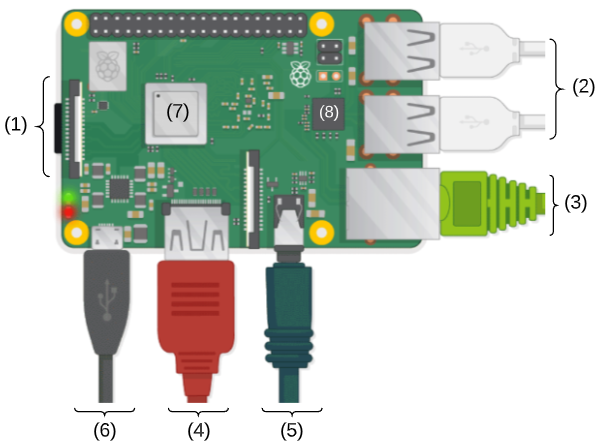
\includegraphics[scale=0.75]{img/raspberry4.png}
 \end{center}
 \caption{Diagrama de componentes de la Raspberry Pi 3. Tomada de \cite{defraspberry} \label{raspberrypng}}
\end{figure}

La Figura anterior permite observar el diagrama de los componentes de una Raspberry Pi y son listados así:
\begin{multicols}{2}
\begin{itemize}
    \item [(1)] Ranura para tarjeta micro SD
    \item [(2)] Puertos de conexión USB
    \item [(3)] Puerto de conexión Ethernet
    \item [(4)] Puerto de conexión HDMI
    \item [(5)] Puerto de conexión de audio (Jack)
    \item [(6)] Puerto de conexión de alimentación
    \item [(7)] Microprocesador
    \item [(8)] Memoria RAM
\end{itemize}
\end{multicols}

\subsection{Sistemas embebidos} \label{subsectionembebidos}

También conocidos como sistemas empotrados, son sistemas de computación diseñados para propósitos especializados de reacción con el entorno, es decir que en tiempo real puedan desempeñar unas pocas funciones dedicadas y al contrario que los computadores, no están diseñados para ser  programados por los usuarios finales. Esto quiere decir que el usuario final no modificará o reemplazará la funcionalidad del sistema al agregar o quitar software. Mas sin embargo, podrá tomar decisiones concernientes a la ejecución de los procesos que éste realice \cite{embebido}. Por lo general, en un sistema embebido, los componentes suelen estar unidos mediante una única placa base que se puede programar mediante lenguajes de programación como ``C'', ``C++'', ``Python'', e incluso ``java''.

\subsubsection{Componentes}

En el listado de componentes centrales de un sistema de este tipo suele encontrarse:

\begin{itemize}
    \item \textbf{Microprocesador:} En términos generales es un circuito integrado perteneciente a la CPU considerado como el ``Cerebro'' en un sistema informático (ver figura \ref{atmegapng}). Este es el encargado de ejecutar el sistema operativo, programas y las aplicaciones de usuario.
    
\begin{figure}[H]
 \begin{center}
 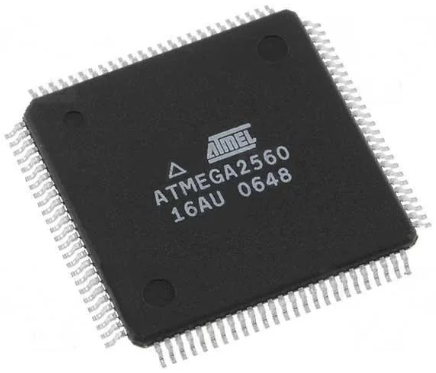
\includegraphics[scale=0.65]{img/atmega.png}
 \end{center}
 \caption{Ejemplar de microprocesador ATMega2560. Tomado de \cite{arduinodef}.
 \label{atmegapng}}
\end{figure}

    \item \textbf{Memoria principal:} Para este tipo de dispositivos comúnmente se emplea una memoria RAM. Es la memoria interna del sistema de cómputo en donde se almacenan las instrucciones y los datos que serán procesados por la CPU con quien se comunica mediante el bus de datos y el bus de direcciones.
    
    \item \textbf{Microcontrolador ($\mu C$):} Es un circuito integrado programable, con la capacidad de ejecutar las ordenes almacenadas en la memoria interna. Típicamente, la arquitectura general de un microcontrolador comercial poseerá dispositivos de entrada y salida como los conversores ADC, temporizadores y buses de interfaz como el $I_2C$ y $CAN$ (ver figura \ref{mucpng}). Los microcontroladores suelen incluir un lenguaje de programación integrado con instrucciones de procesadores especializados como lo es en el caso de Arduino y BASIC.
    
\begin{figure}[H]
 \begin{center}
 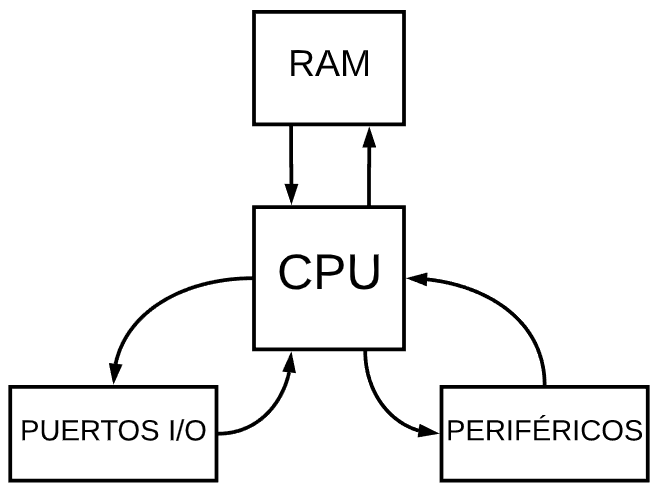
\includegraphics[scale=0.65]{img/muc.png}
 \end{center}
 \caption{Diagrama de comunicación con periféricos. \label{mucpng}}
\end{figure}

    
    A diferencia de un microprocesador, estos pueden ser convertidos en una computadora funcional mediante la conexión de circuitos integrados externos de apoyo y conexión a los sistemas de información y alimentación que requiera. Por su parte, el microprocesador requerirá que otros chips o módulos se encarguen de estas tareas.\\
    
    \item \textbf{Unidad de procesamiento digital de señales (DSP):} Por medio de esta se logra la manipulación matemática y digital de una señal en pro de modificarla, analizarla o mejorarla en algún sentido. Las señales entrantes y salientes pasan por un proceso de conversión analógica $\Longleftrightarrow$ digital mediante los conversores ADC y DAC. Estas unidades se obtienen al interconectar hardware, software e instrucciones optimizadas para aplicaciones numéricas. Gracias a esto, es especialmente útil para aplicaciones de procesamiento y representación de señales analógicas en tiempo real.
\end{itemize}

En resumen, estos componentes reflejan la Unidad de Central de Procesamiento (CPU). En lo que respecta a la visualización de datos se tienen dispositivos de salida como las pantallas LCD, gráficas, o interfaces alfanuméricas.\\

Por último, además de su estructura física, la parte tangible de los sistemas embebidos comprende a los actuadores, que es todo tipo de elemento electrónico que pueda ser manipulado por señales de control; entre los más comunes son los motores de corriente continua mediante pulsos modulados (PWM).

\subsubsection{Sistema de tiempo real}

Son sistemas informáticos de interacción con el entorno físico que reaccionan a estímulos del entorno en  determinados instantes de tiempo ($Inputs$). Según la aplicación se puede tratar de tiempo real crítico (o duro) y acrítico (o suave); respectivamente quiere decir que los tiempos de respuesta pueden determinar si la reacción al estímulo debe realizarse explícitamente en  un intervalo de tiempo específico o no.

Entre los dispositivos más usados para los sistemas de tiempo real crítico y acrítico se puede mencionar a Arduino; en particular, para este último caso y, en algunas ocasiones, para el primer caso.

Debido a su acogida en el mercado, simplicidad de uso y codificación, y su uso en aplicaciones de prototipado y aprendizaje en tareas especializadas, es un gran postor como microcontrolador  en sistemas embebidos. Mediante la conexión de diferentes sensores, módulos y componentes de hardware se pueden lograr tareas funcionales de fácil aplicación y manipulación. Un esquema de ejemplo para un sistema de tiempo real crítico se puede ver en la Figura \ref{esquematico1png}.

\begin{figure}[H]
 \begin{center}
 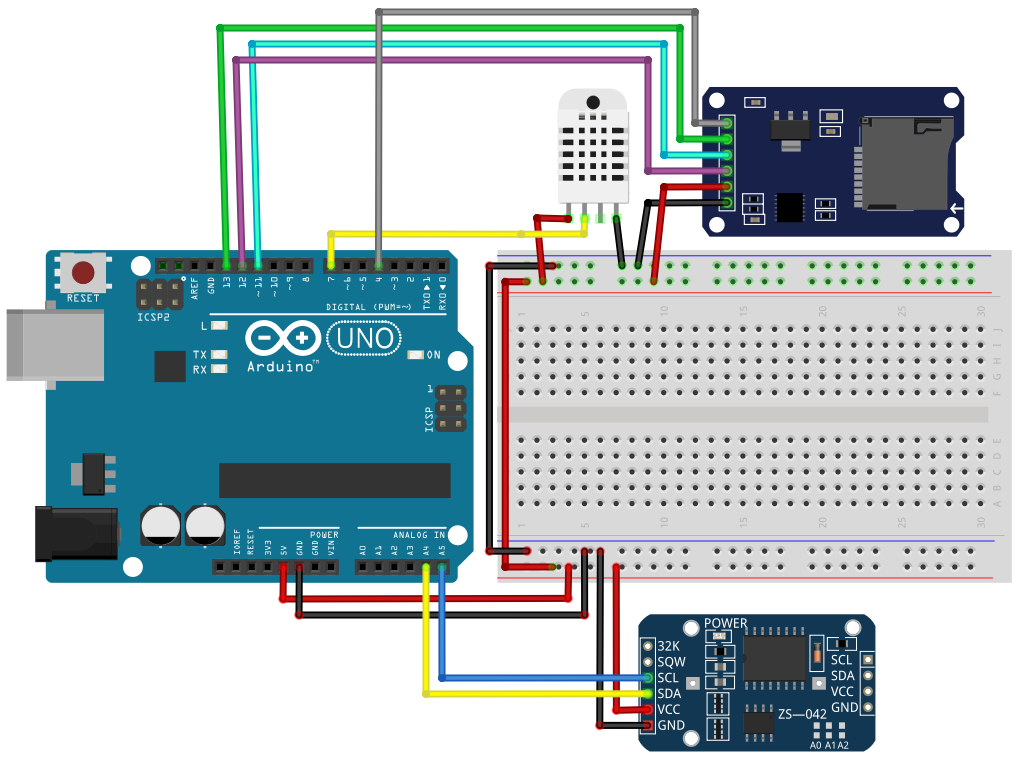
\includegraphics[scale=0.35]{img/esquematico1.png}
 \end{center}
 \caption{Ejemplo de esquemático de conexión de Arduino para medición y registro de temperatura y hora. \label{esquematico1png}}
\end{figure}

% Un ejemplo que ilustra los puntos anteriores es el de un robot que necesita tomar una pieza de una banda sinfín. Si el robot llega tarde, la pieza ya no estará donde debía recogerla, por tanto, el trabajo se llevó a cabo incorrectamente, aunque el robot haya llegado al lugar adecuado. Si el robot llega antes de que la pieza llegue, la pieza aún no estará ahí y el robot puede bloquear su paso.

\subsubsection{Aplicaciones}

Para el desarrollo de aplicaciones con sistemas embebidos y prototipos existen plataformas desarrolladas como Raspberry Pi, Arduino, mbed, BeagleBone, entre otros.\\

Los programas de sistemas embebidos se enfrentan usualmente a tareas de procesamiento en tiempo real por lo que para ejemplificar aplicaciones de estos sistemas electrónicos se mencionan las siguientes:

\begin{itemize}
    \item  \textbf{Sistemas automatizados de alimentación para vacas de alta producción de leche}
    En este trabajo de grado, se utiliza un sistema electrónico que se encarga de registrar si un animal ha ingerido su porción fija de alimento en su totalidad, y se encarga de registrar  el restante en caso que se presente esa situación. Para mayor información ver \cite{aguero}.  
    \item  \textbf{Dispensador automático de comida para mascotas, programable y controlado remotamente}
    En este trabajo de grado de la Universidad del Valle se utiliza un microcontrolador $ATMEGA644$ para procesar las indicaciones  y activar los mecanismos de dosificación de alimento en porciones y horas determinadas. Tomado de \cite{univalle}.\\
    \item  \textbf{Maquinaria de pesado industrial y doméstica} 
    Entre las aplicaciones más comunes de un sistema embebido sencillo se encuentran las básculas de pesaje tanto doméstico como industrial.
    \item  \textbf{Impresoras 3D}
    En la actualidad es posible fabricar impresoras 3D sencillas mediante el uso de sistemas embebidos con micro controladores como Arduino y módulos adicionales de control para el manejo de los motores que maniobran en el espacio de impresión.
    \item  \textbf{Robótica}
    El uso de estos sistemas es altamente usado en la industria para tareas sistematizadas como el control y la automatización de procesos en sistemas de control de lazo cerrado y sobre todo en sistemas de tiempo real crítico como en las cintas transportadoras.
\end{itemize}

% \textbf{BITÁCORA DEL TIEMPO 12 SEPTIEMBRE 2019 8:30PM 
% Hacer la comparacion entre ardino y la resperry pi cuando mencione la parte de escoger al microprocesador pero eso sería mas adelante en el capitulo 5 o 6}

% \subsubsection{Microprocesadores}
